


%
% How to fix the Underfull \vbox badness has occurred while \output is active on my memoir chapter style?
% https://tex.stackexchange.com/questions/387881/how-to-fix-the-underfull-vbox-badness-has-occurred-while-output-is-active-on-m
%

% ---

\lang
% {\chapter[Page not filled]{Since this page is not being completely filled, it is generating the bottom bottom of the page}}
% {\chapter[Página não gerada]{Como esta página não está sendo completamente preenchida, ele está gerando a caixa inferior inferior da página}}
% ---


% Multiple-language document - babel - selectlanguage vs begin/end{otherlanguage}
% https://tex.stackexchange.com/questions/36526/multiple-language-document-babel-selectlanguage-vs-begin-endotherlanguage
\begin{otherlanguage*}{brazil}

\chapter{Manual de uso LTI Beecrowd no Moodle}
\label{manual:uso-lti}

\section{Utilizar LTI do Beecrowd já configurada no Moodle}

Este Manual mostra como o professor cria uma atividade Beecrowd no Moodle, como um aluno acessa essa atividade, e como o professor pode transferir as notas do Beecrowd para o Moodle.

\subsection{Criando a atividade}

\begin{enumerate}
    \item Entre em modo edição
    \item Vá em adicionar uma atividade ou recurso:

    \begin{figure}[H]
        \centering
            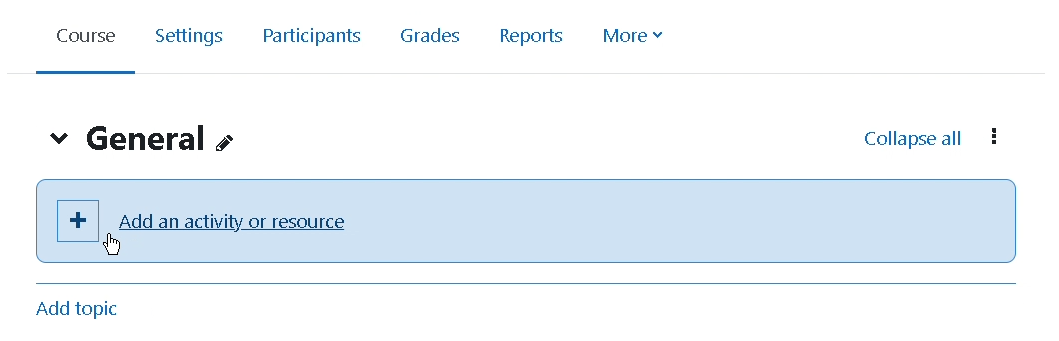
\includegraphics[scale=0.45]{pictures/apendices/apendice_b_1.png}
    \end{figure}

    \item Selecione a atividade “beecrowd”

    \begin{figure}[H]
        \centering
            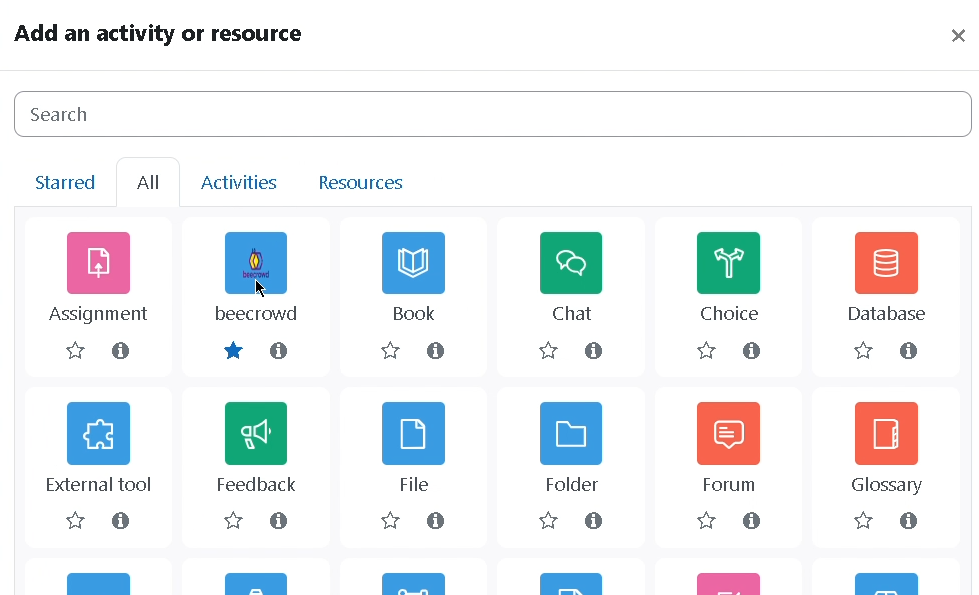
\includegraphics[scale=0.45]{pictures/apendices/apendice_b_2.png}
    \end{figure}

    \item Na página que abrir:

    \begin{enumerate}
        \item Em \textbf{General} > \textbf{Activity Name}, escreva o nome da atividade - como essa primeira vai ser para uso do professor, para entrar no Beecrowd Academic, você pode escolher um nome tipo \textit{“Acesso ao Beecrowd Acadêmico”};
        \item Em \textbf{Grade} > \textbf{Type}, selecione \textit{None};
        \item Em \textbf{Common module settings} > \textbf{Availability}, selecione \textit{“Hidden on Course Page”};
        \item Clique em \textbf{Save and return to course}.
    \end{enumerate}

    \begin{figure}[H]
        \centering
            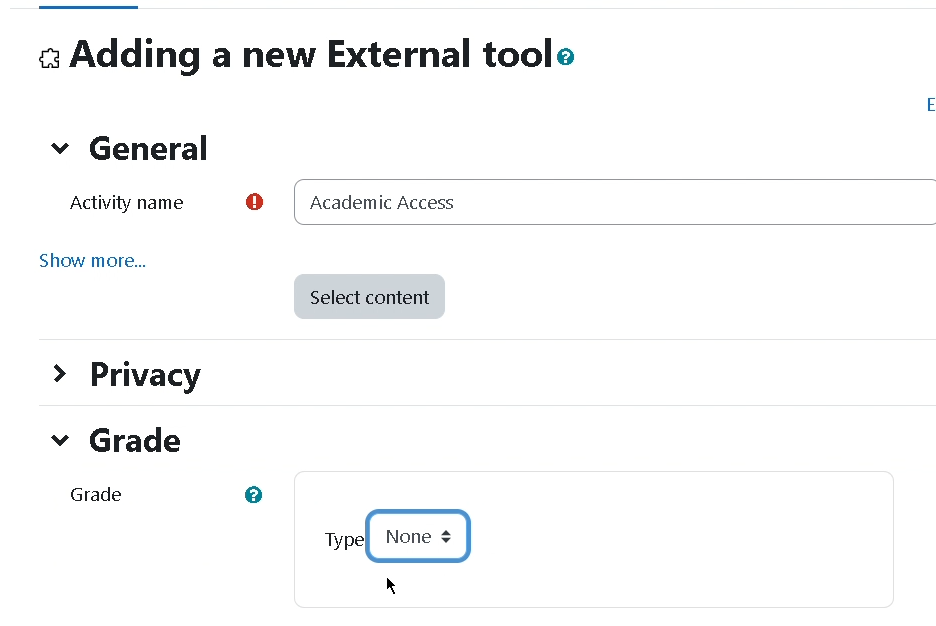
\includegraphics[scale=0.425]{pictures/apendices/apendice_b_3.png}
    \end{figure}

    \begin{figure}[H]
        \centering
            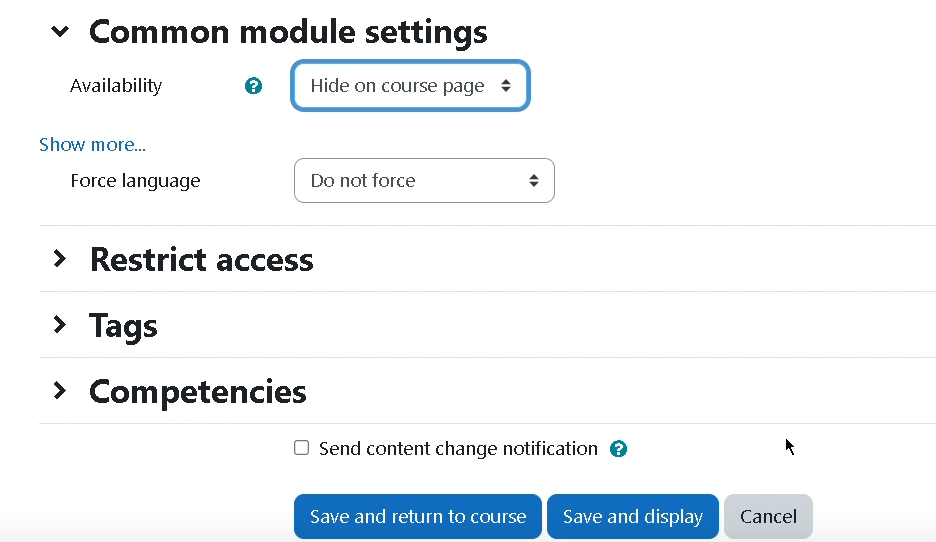
\includegraphics[scale=0.425]{pictures/apendices/apendice_b_4.png}
    \end{figure}

    \item Agora, a atividade que você criou vai aparecer na página do curso. Clique nela.

    \begin{figure}[H]
        \centering
            
\includegraphics[scale=0.3]{pictures/apendices/apendice_b_5.png}
    \end{figure}

    \item Você vai ser redirecionado para a página do Beecrowd Academic. Caso você já esteja logado, vai aparecer a lista de suas disciplinas.    
    \begin{figure}[H]
        \centering
            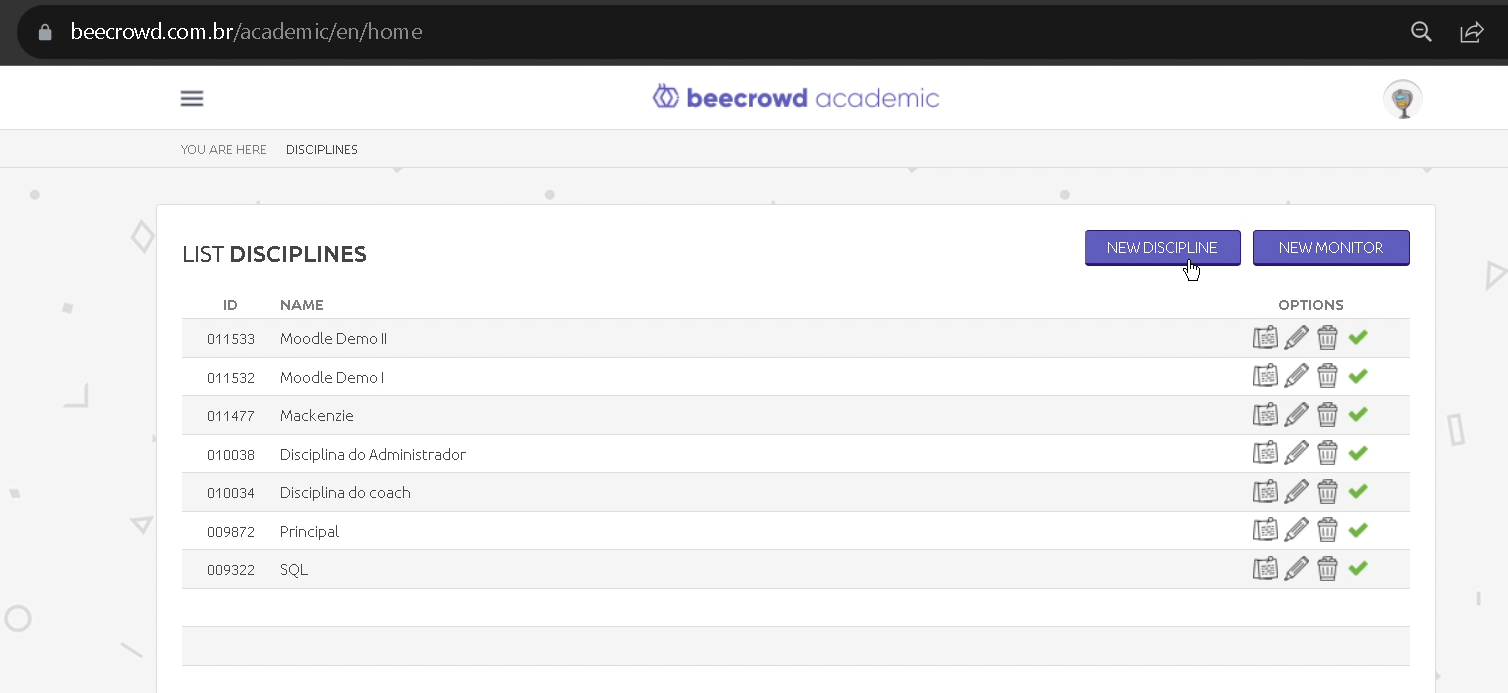
\includegraphics[scale=0.35]{pictures/apendices/apendice_b_6.png}
    \end{figure}

    Você pode criar uma disciplina, ou selecionar uma disciplina já existente. Para cada disciplina, você pode criar tarefas, e, para cada tarefa, você pode selecionar diferentes questões, e arrumar outras configurações, como data de início, de fim, etc (Veja as imagens da próxima página).

    Criar ou editar tarefa:

    \begin{figure}[H]
        \centering
            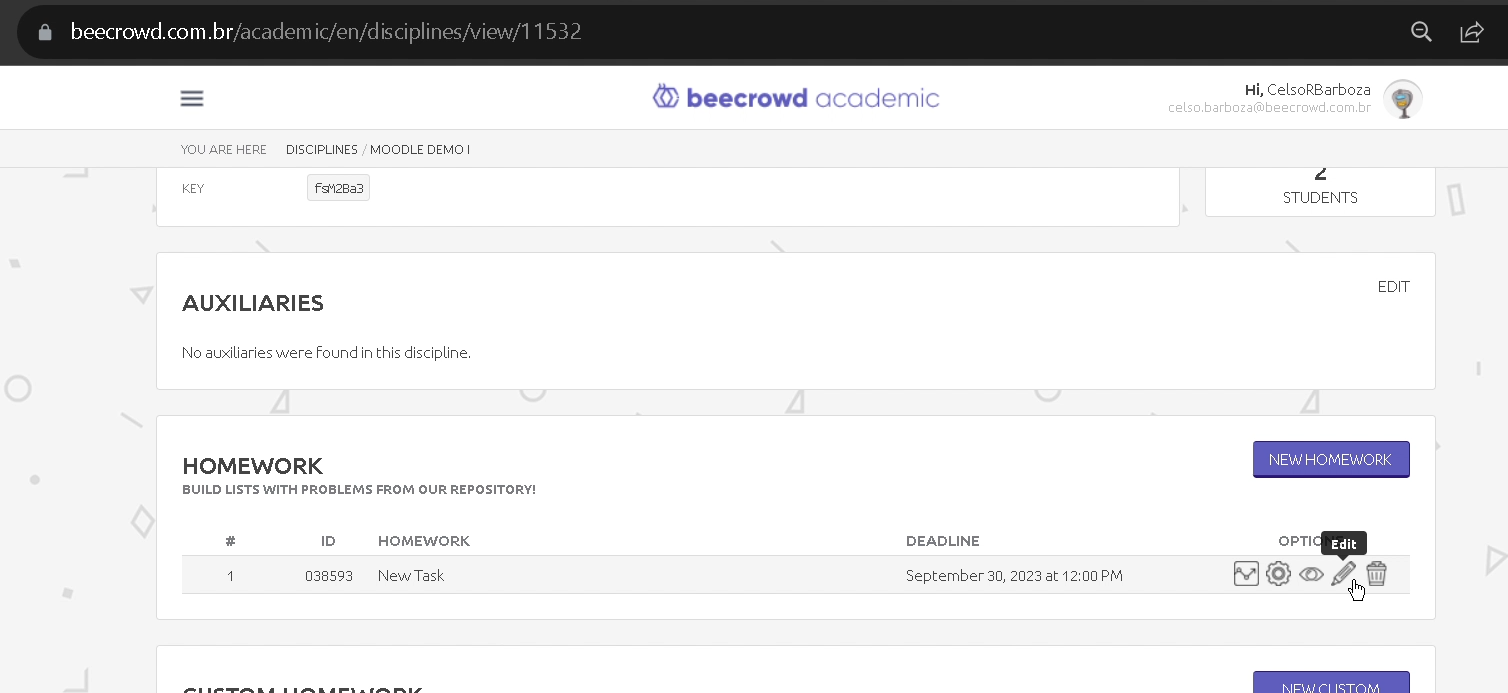
\includegraphics[scale=0.35]{pictures/apendices/apendice_b_7.png}
    \end{figure}

    Editando a tarefa:

    \begin{figure}[H]
        \centering
            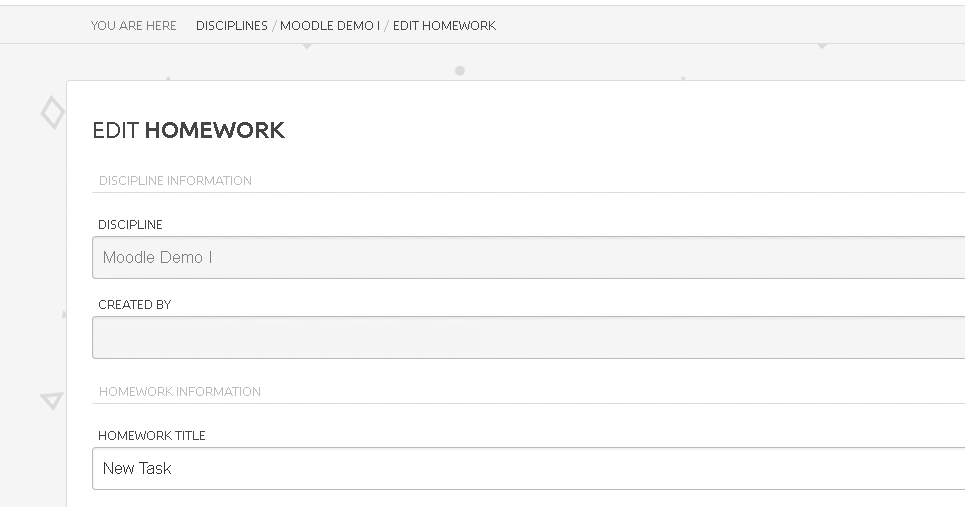
\includegraphics[scale=0.45]{pictures/apendices/apendice_b_8.png}
    \end{figure}

    Selecionando questões:

    \begin{figure}[H]
        \centering
            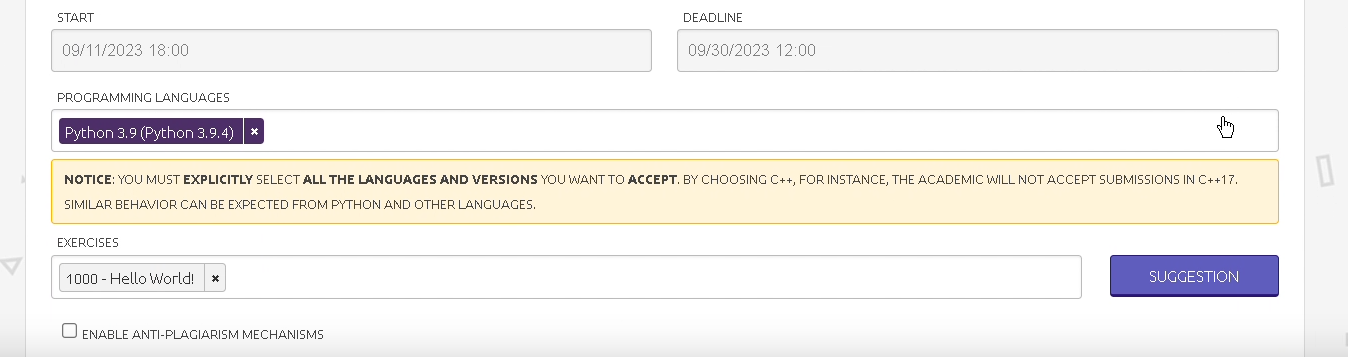
\includegraphics[scale=0.3]{pictures/apendices/apendice_b_9.png}
    \end{figure}
    
    \item Agora que você tem a disciplina com a tarefa desejada, volte ao Moodle e clique para adicionar uma atividade ou recurso:

    \begin{figure}[H]
        \centering
            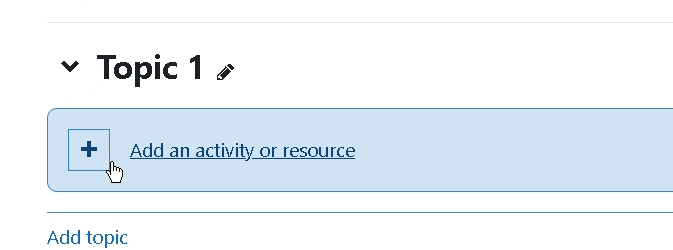
\includegraphics[scale=0.3]{pictures/apendices/apendice_b_10.png}
    \end{figure}

    \item Selecione a atividade Beecrowd:

    \begin{figure}[H]
        \centering
            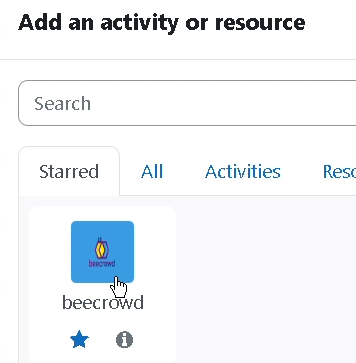
\includegraphics[scale=0.45]{pictures/apendices/apendice_b_11.png}
    \end{figure}

    \item Clique em “Selecionar conteúdo”:

    \begin{figure}[H]
        \centering
            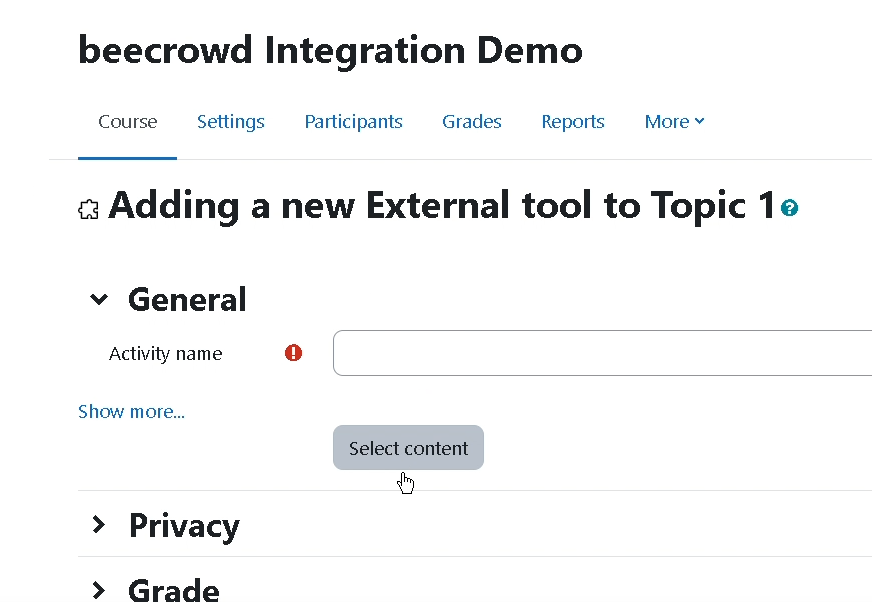
\includegraphics[scale=0.45]{pictures/apendices/apendice_b_12.png}
    \end{figure}

    \item Selecione a Disciplina criada no Beecrowd Academic:

    \begin{figure}[H]
        \centering
            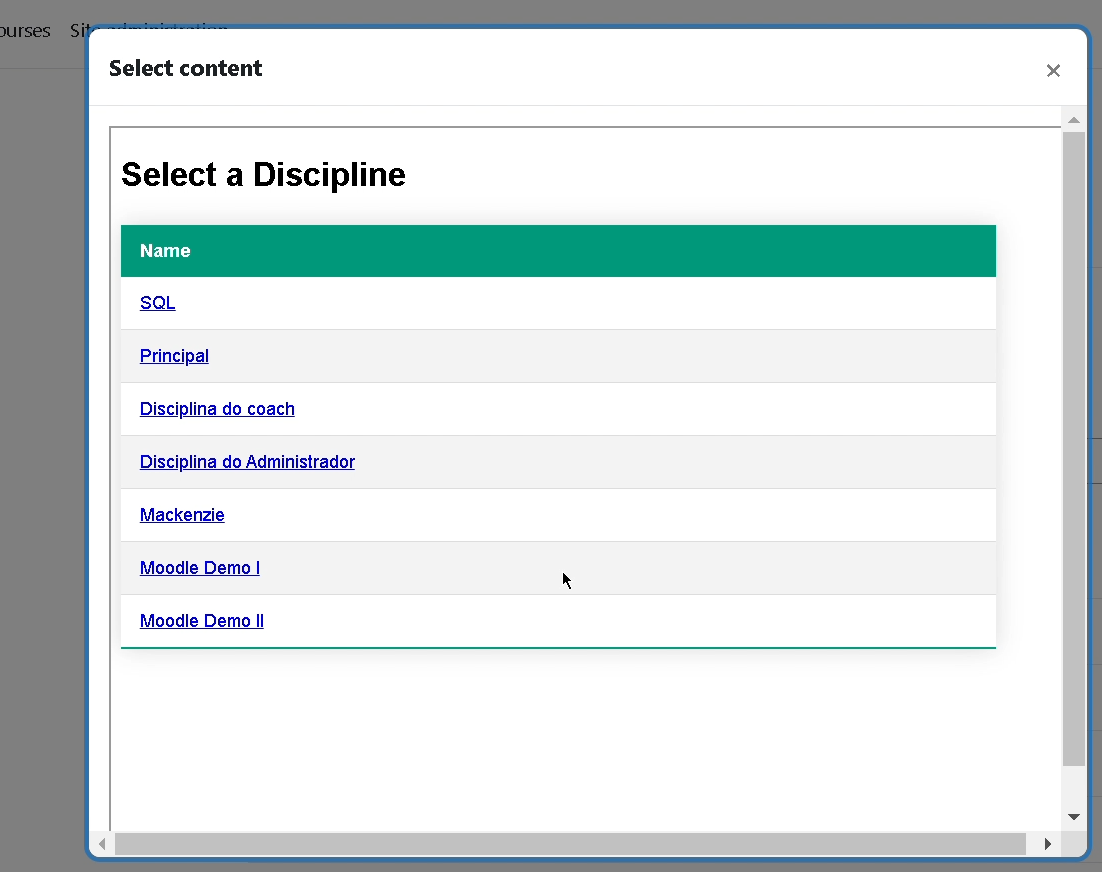
\includegraphics[scale=0.4]{pictures/apendices/apendice_b_13.png}
    \end{figure}

    \item Selecione a tarefa criada no Beecrowd Academic:

    \begin{figure}[H]
        \centering
            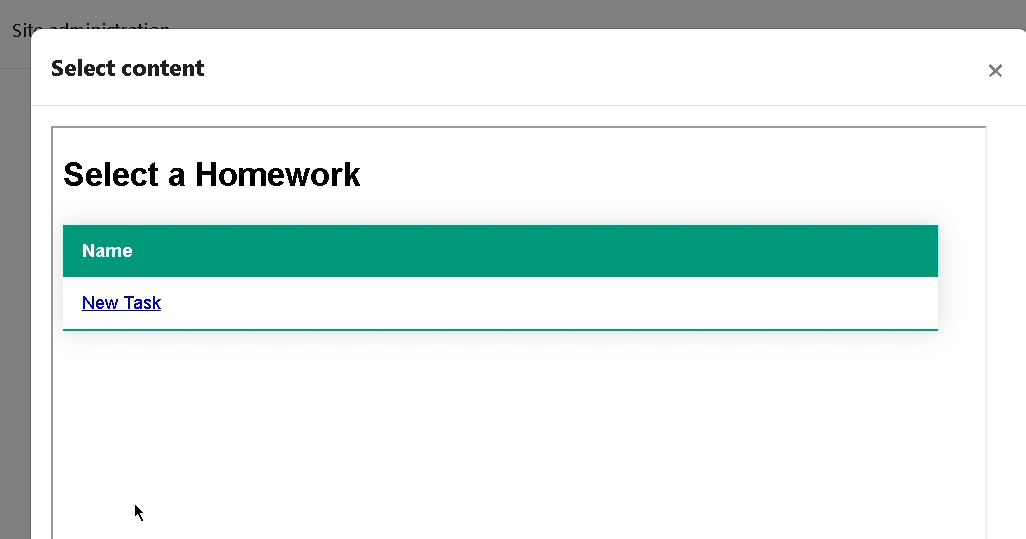
\includegraphics[scale=0.4]{pictures/apendices/apendice_b_14.png}
    \end{figure}

    Vai aparecer uma mensagem de confirmação que a tarefa foi selecionada com sucesso:

    \begin{figure}[H]
        \centering
            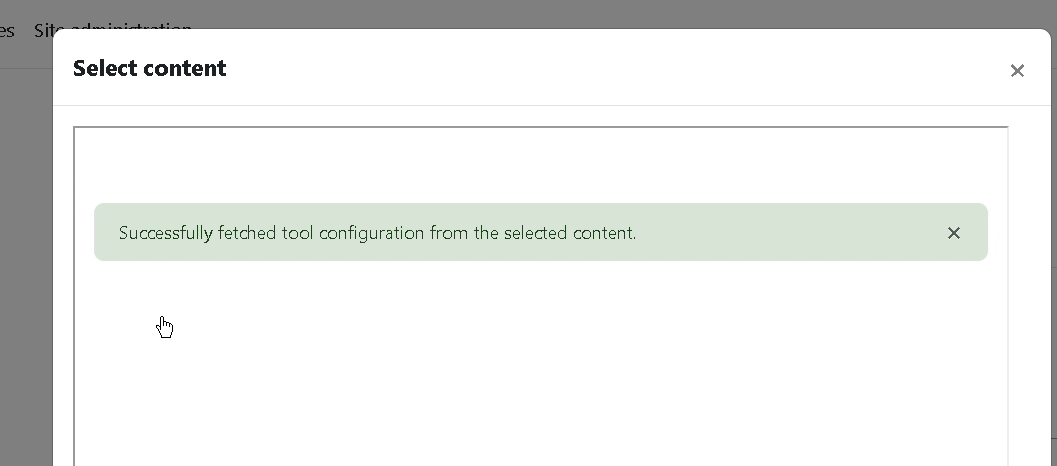
\includegraphics[scale=0.4]{pictures/apendices/apendice_b_15.png}
    \end{figure}

    \item Você vai ser redirecionado de volta para a tela anterior, e agora é só clicar em “Save and return do course”:

    \begin{figure}[H]
        \centering
            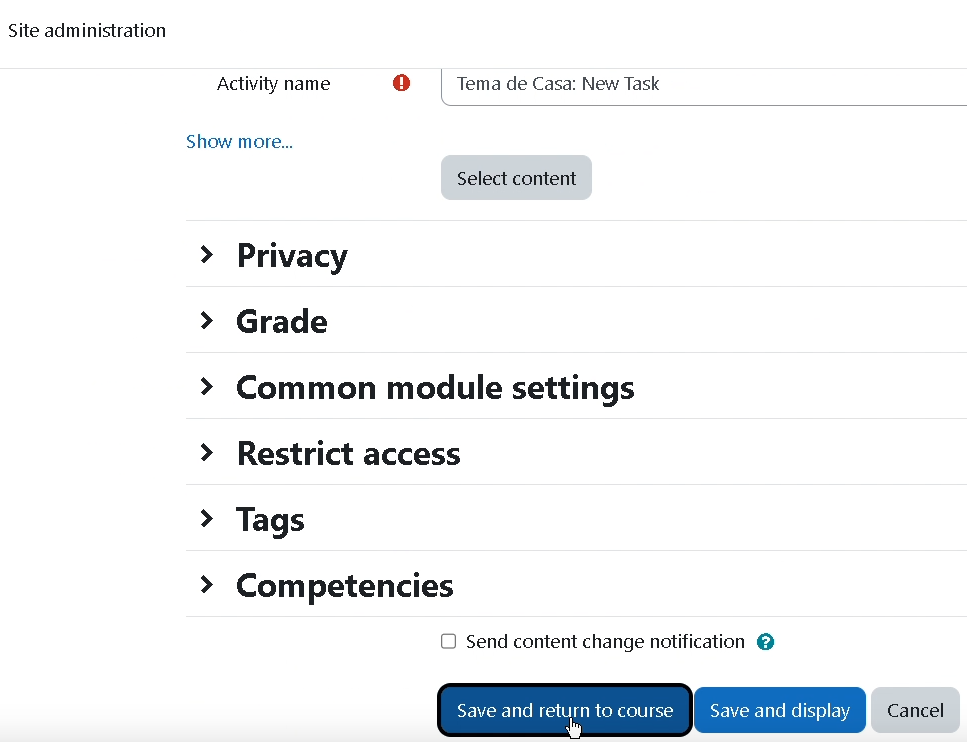
\includegraphics[scale=0.35]{pictures/apendices/apendice_b_16.png}
    \end{figure}

    Agora a tarefa aparecerá dessa forma na página do curso:

    \begin{figure}[H]
        \centering
            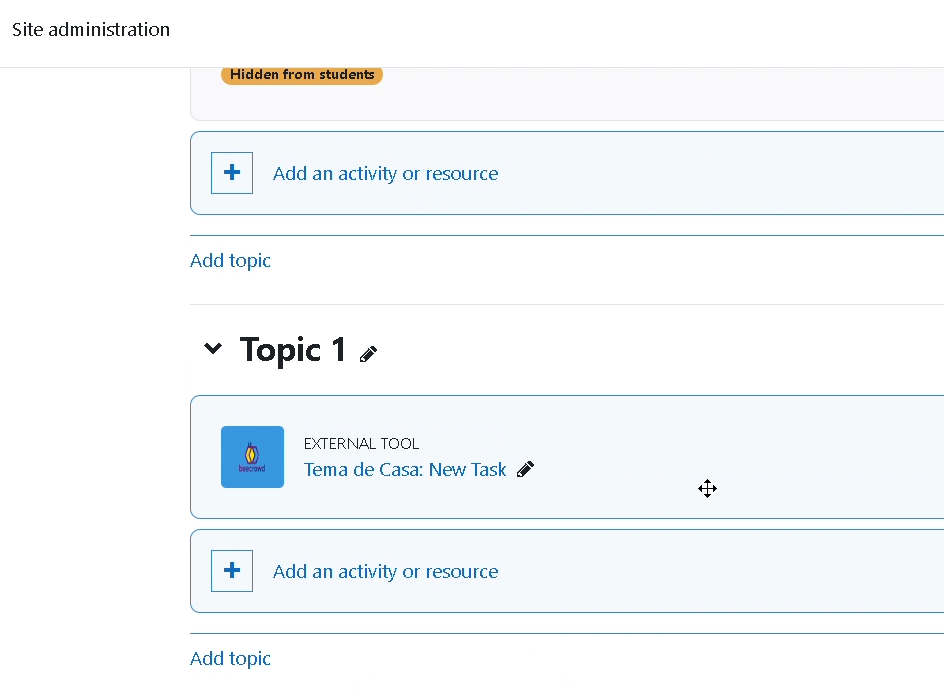
\includegraphics[scale=0.4]{pictures/apendices/apendice_b_17.png}
    \end{figure}
\end{enumerate}

\end{otherlanguage*}

\clearpage

\subsection{Entrando como aluno}

\begin{enumerate}
    \item O aluno clica na tarefa do Beecrowd, criada pelo professor:

    \begin{figure}[H]
        \centering
            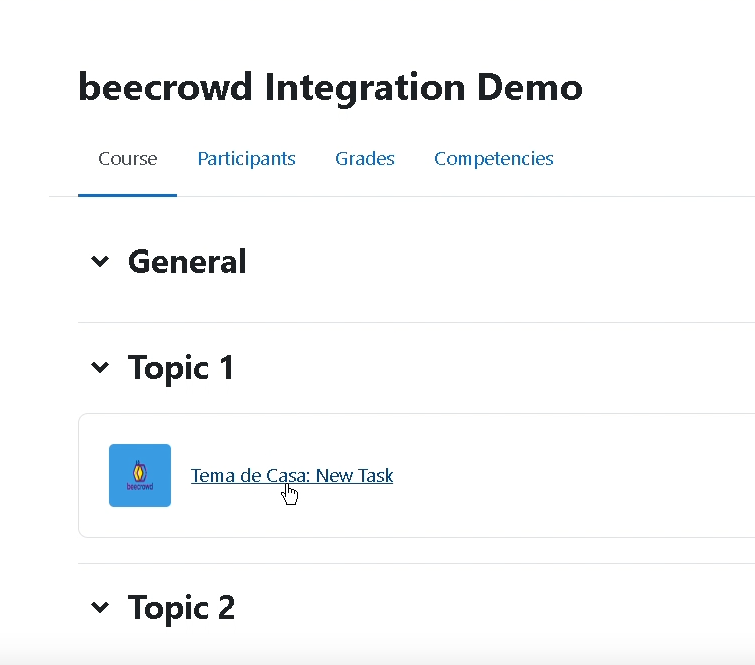
\includegraphics[scale=0.425]{pictures/apendices/apendice_b_18.png}
    \end{figure}

    \item O aluno é direcionado à tarefa do Beecrowd, sem precisar criar um usuário, e já pode começar a resolver os exercícios da tarefa:

    \begin{figure}[H]
        \centering
            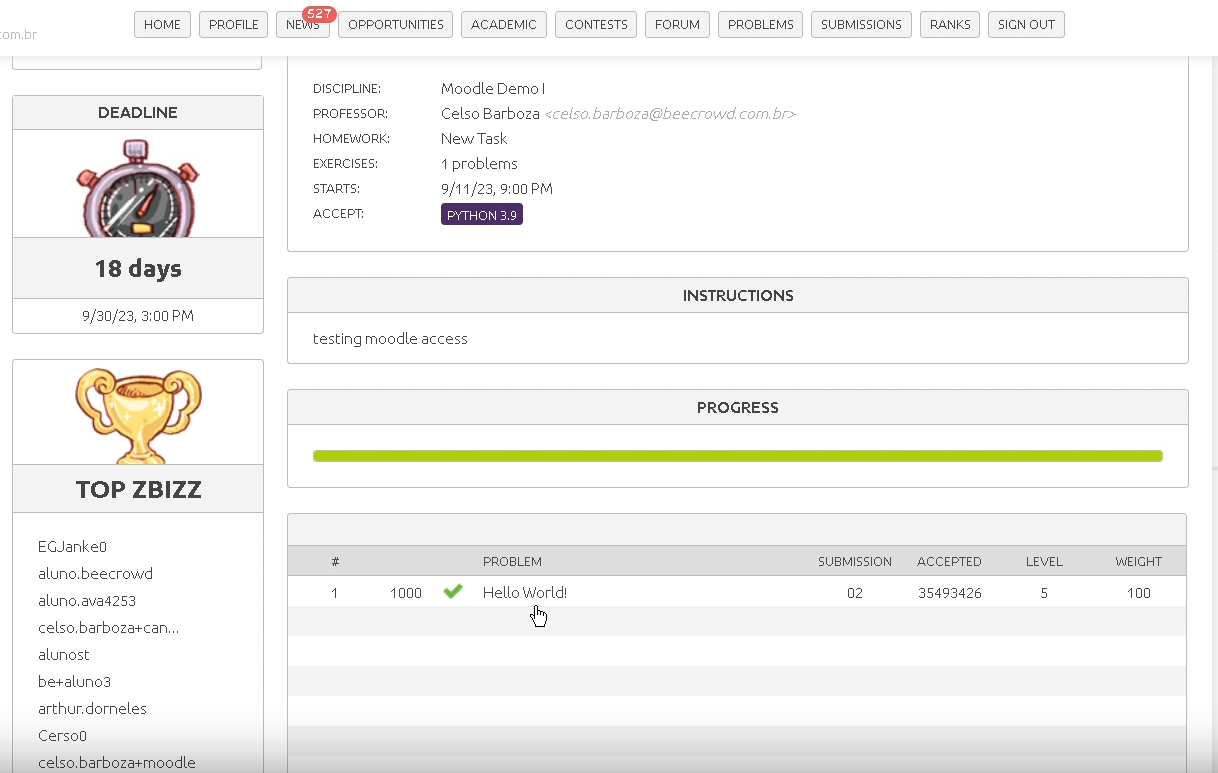
\includegraphics[scale=0.5]{pictures/apendices/apendice_b_19.png}
    \end{figure}

    Resolvendo um exercício:

    \begin{figure}[H]
        \centering
            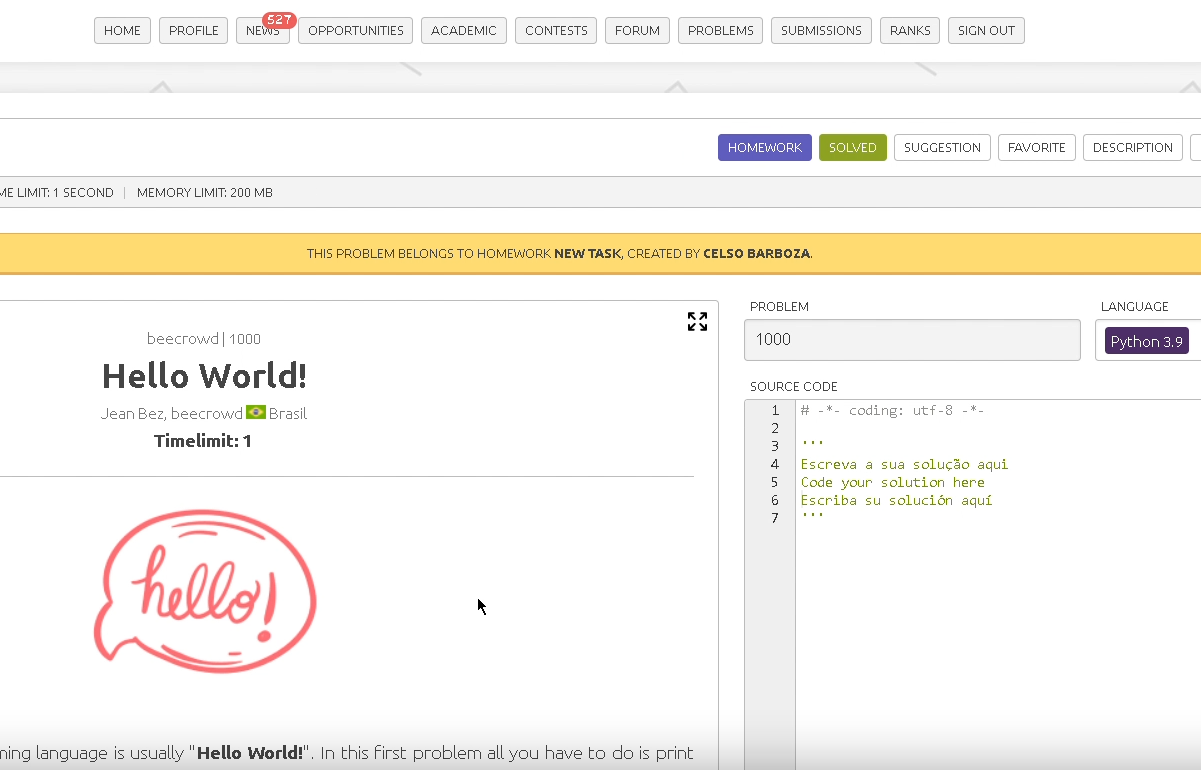
\includegraphics[scale=0.375]{pictures/apendices/apendice_b_20.png}
    \end{figure}

    Digita o código e clica em Submit:

    \begin{figure}[H]
        \centering
            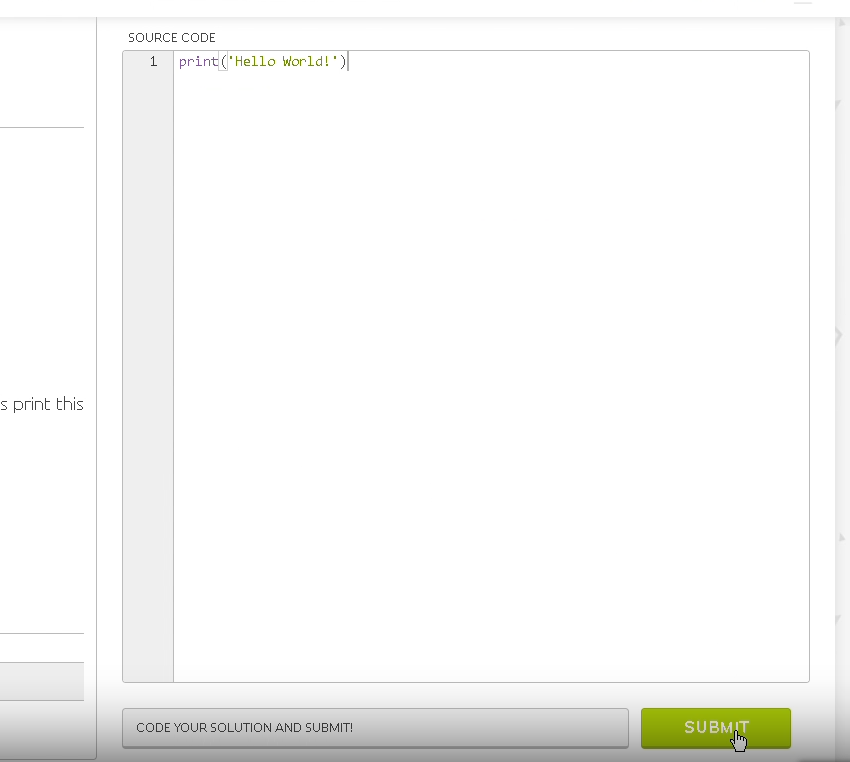
\includegraphics[scale=0.425]{pictures/apendices/apendice_b_22.png}
    \end{figure}

    O código é avaliado pelo juíz online da plataforma:

    \begin{figure}[H]
        \centering
            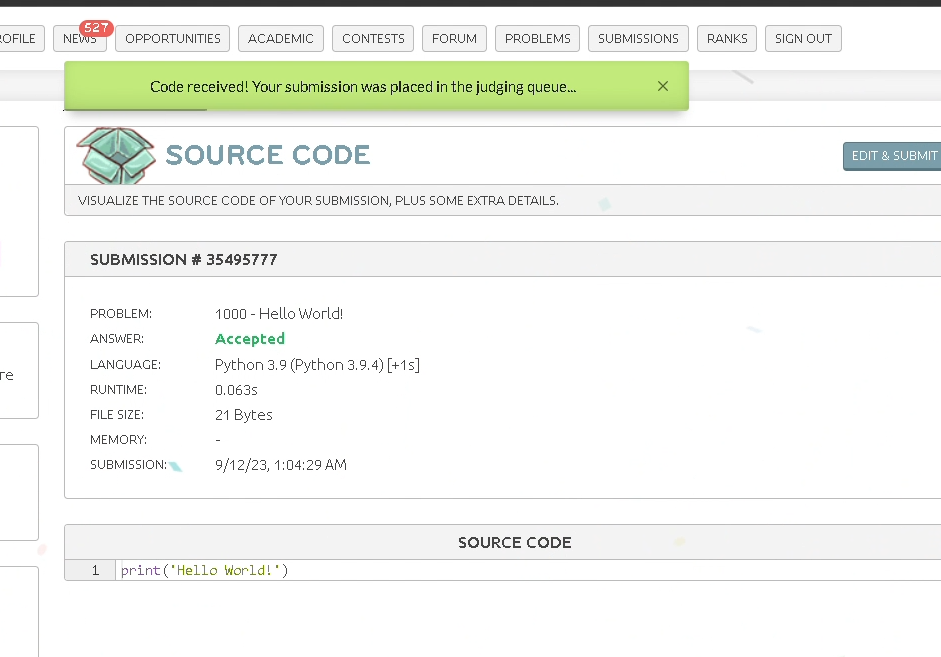
\includegraphics[scale=0.45]{pictures/apendices/apendice_b_23.png}
    \end{figure}
\end{enumerate}

\clearpage

\subsection{Notas}

\begin{enumerate}
    \item Após seguir os passos anteriores descritos nesse documento, o professor pode clicar na tarefa do Beecrowd que ele criou para os alunos:

    \begin{figure}[H]
        \centering
            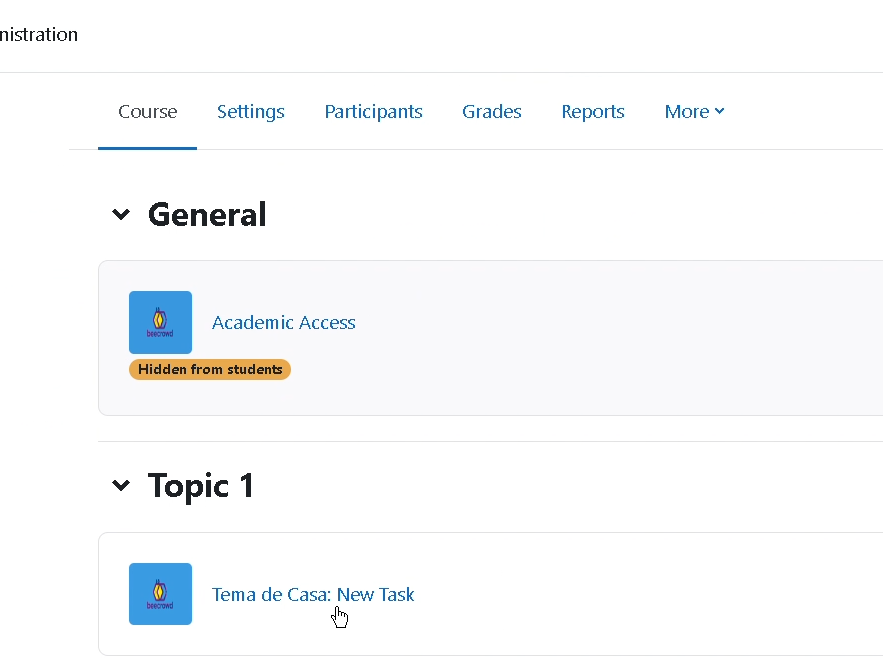
\includegraphics[scale=0.4]{pictures/apendices/apendice_b_24.png}
    \end{figure}

    \item O professor pode visualizar quem respondeu as questões, e, ao clicar em \textbf{“Send Grades”}, as notas são enviadas para o Moodle, e o professor consegue visualizar as notas lá:

    Página da tarefa no Beecrowd Academic:

    \begin{figure}[H]
        \centering
            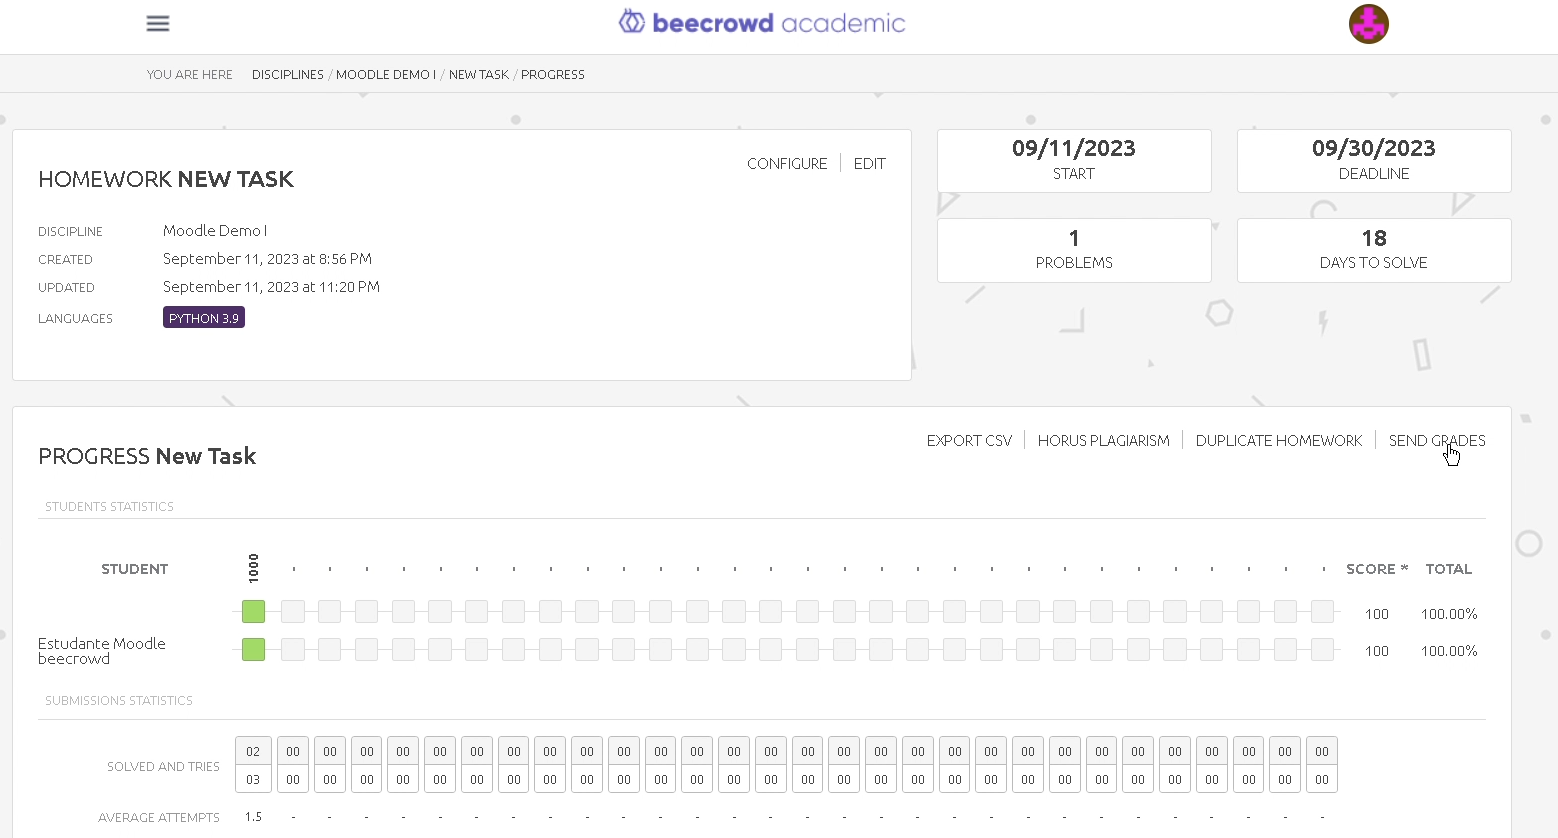
\includegraphics[scale=0.385]{pictures/apendices/apendice_b_25.png}
    \end{figure}

    Clica em “Send Grades”:

    \begin{figure}[H]
        \centering
            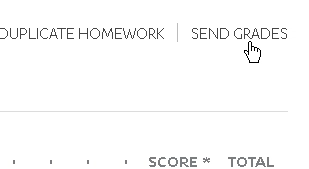
\includegraphics[scale=0.5]{pictures/apendices/apendice_b_26.png}
    \end{figure}

    Mensagem de sucesso que as notas foram enviadas:

    \begin{figure}[H]
        \centering
            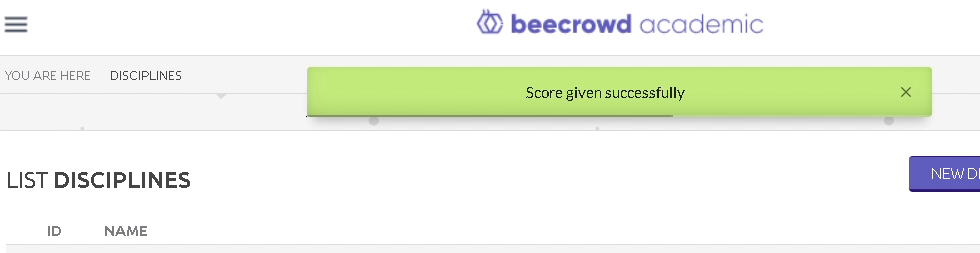
\includegraphics[scale=0.43]{pictures/apendices/apendice_b_27.png}
    \end{figure}

    Notas agora estão moodle:

    \begin{figure}[H]
        \centering
            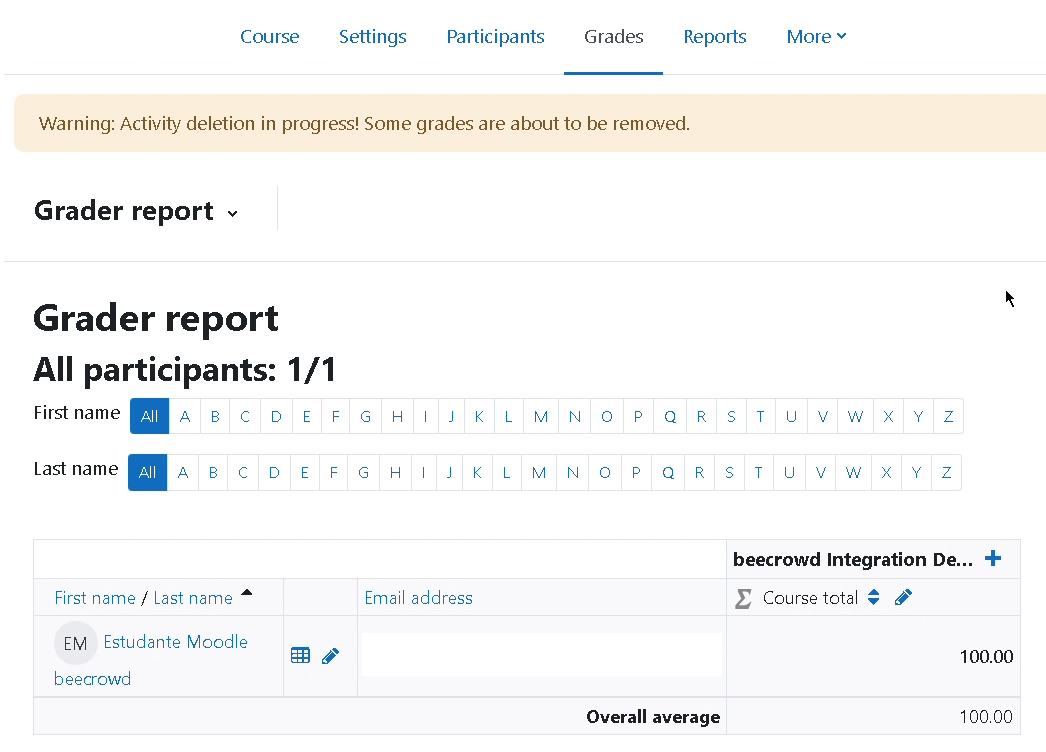
\includegraphics[scale=0.43]{pictures/apendices/apendice_b_28.png}
    \end{figure}

\end{enumerate}

\end{otherlanguage*}


